% This is auto-generated file: do not edit!
% Exported from microMathematics Plus, version 2.22.1


Ahora trazamos varias funciones dadas
en el sistema de coordenadas polares.
Cada punto de este sistema está
determinado por una distancia r desde
el origen y el ángulo f desde el eje
x.
\begin{center}\begin{tabular}{c} 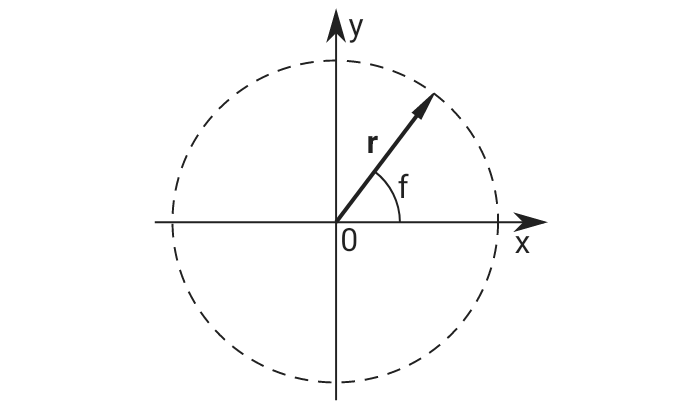
\includegraphics[width=0.45\textwidth]{graphics/polar_plot_fig1.png} \end{tabular}\end{center}

El ángulo f es nuestra variable
independiente que se cambia de la
siguiente manera:
\begin{center}\begin{tabular}{c}
  $f := \left[ 0.01,\, 0.05 \,..\, 300 \right]$
\end{tabular}\end{center}

La distancia r(f) es nuestra variable
dependiente. Teniendo un par de f y r,
podemos transformarla en las
coordenadas cartesianas x e y usando
funciones de seno y coseno:
\begin{center}\begin{tabular}{cc}
  $x(r) := r \cdot cos \left( f\right) $ &
  $y(r) := r \cdot sin \left( f\right) $ \cr
\end{tabular}\end{center}

\subsection{Un caracol}

Definiremos nuestra función polar en
tres pasos. La primera expresión
define una ''rueda'':
\begin{center}\begin{tabular}{ccc}
  $A := 1.1$ &
  $B := 1.271$ &
  $q := 2$ \cr
\end{tabular}\end{center}
\begin{center}\begin{tabular}{c}
  $r1(f) := A + 2 \cdot {sin \left( B \cdot f\right) }^{q}$
\end{tabular}\end{center}

Para trazar esta función, añadimos el
cuadro gráfico usando el botón ''Nuevo
elemento'' en la barra de acciones o el
botón ''Añadir gráfica de la función''
de la barra de herramientas:
\begin{center}\begin{tabular}{c} 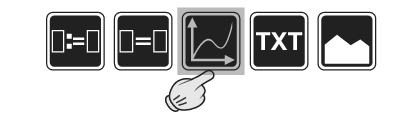
\includegraphics[width=0.45\textwidth]{graphics/polar_plot_fig2.png} \end{tabular}\end{center}

En lugar de f y r, usaremos aquí reglas
previamente definidas de la
transformación para x e y, donde r1(f)
se utiliza como un argumento simbólico
para estas reglas:
\begin{center}\begin{tabular}{c} 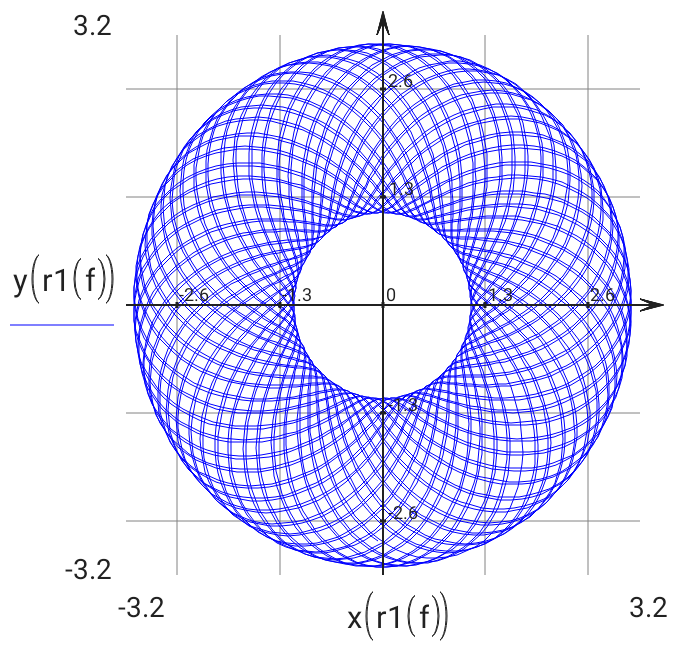
\includegraphics[width=0.45\textwidth]{graphics/polar_plot_fig3.png} \end{tabular}\end{center}

A continuación, podemos modificar esta
rueda a continuación:
\begin{center}\begin{tabular}{c}
  $r2(f) := A + 2 \cdot {sin \left( B \cdot f + 1 \cdot r1 \left( f\right) \right) }^{q}$
\end{tabular}\end{center}
\begin{center}\begin{tabular}{c} 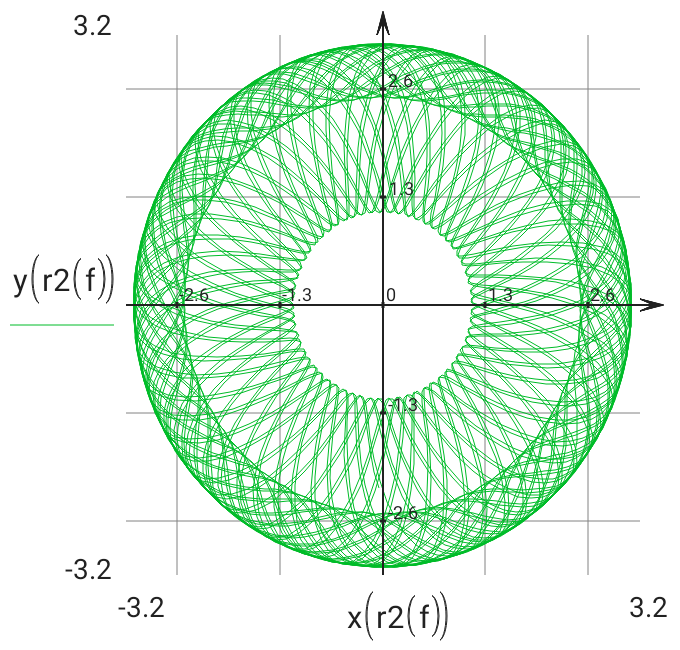
\includegraphics[width=0.45\textwidth]{graphics/polar_plot_fig4.png} \end{tabular}\end{center}

Finalmente, escalamos la última función
r2(f) usando un conversión de flotador
a número para parecer a una función de
paso. Como resultado, obtenemos un
bonito caracol:
\begin{center}\begin{tabular}{c}
  $r(f) := r2 \left( f\right)  \cdot floor \left( f\right)  / 10$
\end{tabular}\end{center}
\begin{center}\begin{tabular}{c} 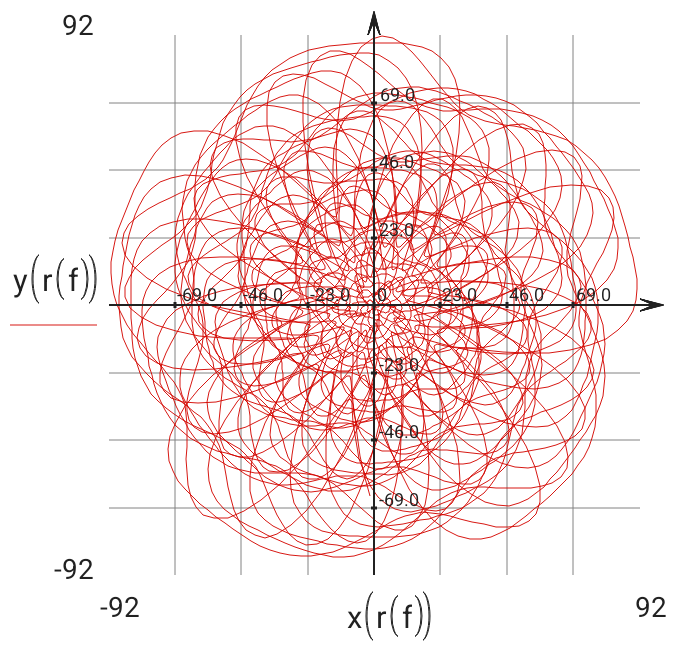
\includegraphics[width=0.45\textwidth]{graphics/polar_plot_fig5.png} \end{tabular}\end{center}

\subsection{Arce japonés}

El arce japonés es bien conocido por
sus atractivas formas de hojas y
colores. Tal hoja puede ser descrita
matemáticamente y trazada como una
curva en el sistema de coordenadas
polares:
\begin{center}\begin{tabular}{c}
  $f := \left[ 0.01,\, 0.02 \,..\, 100 \right]$
\end{tabular}\end{center}
\begin{center}\begin{tabular}{cc}
  $x(r) := r \cdot cos \left( f\right) $ &
  $y(r) := r \cdot sin \left( f\right) $ \cr
\end{tabular}\end{center}
\begin{center}\begin{tabular}{c}
  $s1(f) := \left( 1 + sin \left( f\right)  \right) \cdot \left( 1 - 0.9 \cdot  \left| sin \left( 4 \cdot f\right)  \right|  \right)$
\end{tabular}\end{center}
\begin{center}\begin{tabular}{c}
  $s2(f) := 0.9 + 0.05 \cdot cos \left( 200 \cdot f\right) $
\end{tabular}\end{center}
\begin{center}\begin{tabular}{c}
  $r(f) := floor \left( f\right)  \cdot s1 \left( f\right)  \cdot s2 \left( f\right)  + random \left( 2\right)  - 1$
\end{tabular}\end{center}
\begin{center}\begin{tabular}{c} 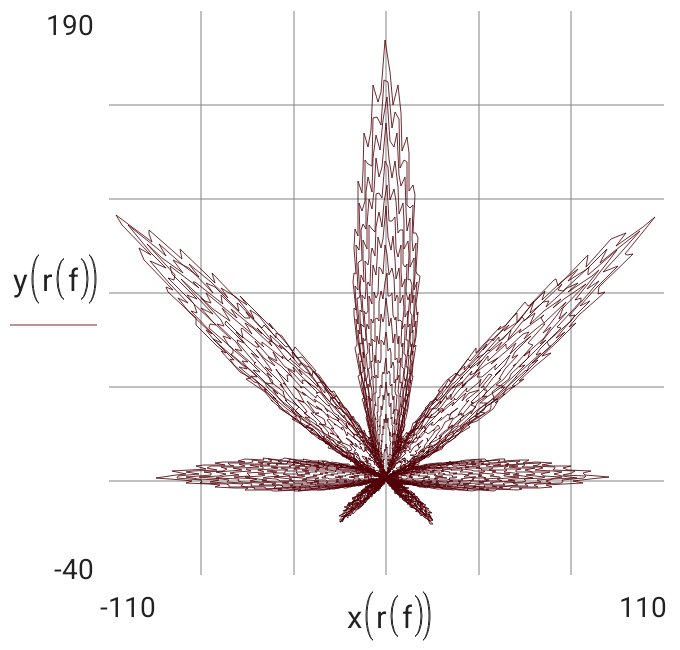
\includegraphics[width=0.45\textwidth]{graphics/polar_plot_fig6.png} \end{tabular}\end{center}

http://es.wikipedia.org/wiki/Acer\_palmatum